\documentclass[a4j,fleqn,dvipdfmx,uplatex]{jsarticle}

\usepackage{sice-si}

\usepackage{epic,eepic}
\usepackage[dvipdfmx]{graphics}
\usepackage[dvipdfmx]{graphicx}
\usepackage[dvipdfmx]{color}
% \usepackage{fancyhdr} % ヘッダフッタの罫線と文字出力
% \pagestyle{fancy} % ヘッダフッタの罫線と文字出力(fancyhdrパッケージとセット)
\usepackage{amsmath} % 数式用
\usepackage{amssymb}
\usepackage{tabularx}
\usepackage{enumerate}
\usepackage{txfonts}
\usepackage{url}
% \usepackage{bm}
\usepackage[subrefformat=parens]{subcaption}
\captionsetup{compatibility=false}

% 図表参照に章番号付加 章をまたいでの参照は不可
\newcommand{\figref}[1]{Fig.\ \ref{#1}}
\newcommand{\tableref}[1]{Table.\ \ref{#1}}

% 章番号の後調整
\newcommand{\secref}[1]{\ref{#1}\hspace{0.2zw} 章}
% 節番号の後調整
\newcommand{\subsecref}[1]{\ref{#1}\hspace{0.2zw} 節}


\begin{document}
%
% タイトルと著者名
\title{FTE新入社員課題報告書\\[1.5mm]本社屋上室外機における\\散水システム導入および比較検討} % 和文タイトル
\name{○高橋 京佑, 小坂 丞, 仲野 茂翠, 設樂 日和, 𠮷岡 拓海, 渡辺 夏芽, 
\\中村 天音, 塚田 浩貴, 青木 昇, 吉川 唯希, 佐藤 央都, 阪田 悠} % 著者名

\etitle{Introduction and Comparison of Watering System \\for Condensing Unit on the office rooftop} % 英文タイトル
\ename{\small○KEISUKE Takahashi, TASUKU Kosaka, MOTOAKI Nakano, HINOWA Shidara, TAKUMI Yoshioka, NATSUME Watanabe, \\
AMANE Nakamura, HIROTAKA Tsukada, NOBORU Aoki, ITSUKI Yoshikawa, HIROTO Sato, YU Sakata}	%著者名(英)
%%%%%%%%%%%%%%%%%%%%%%%%%%%%%%%%%%%%%%%%%%%%%%%%%%%%%%%%%%%%%%%%%%%%%%%%%%%%%%%%%%%%%%%%%%%%%%%%%%%
% アブストラクト
\abst{}

% タイトルの出力
\maketitle
%%%%%%%%%%%%%%%%%%%%%%%%%%%%%%%%%%%%%%%%%%%%%%%%%%%%%%%%%%%%%%%%%%%%%%%%%%%%%%%%%%%%%%%%%%%%%%%%%%%
% 本文
\section{序論}\label{sec1}
\subsection{背景}\label{background}
近年, 地球温暖化の影響のため, 日本全国の気温は上昇傾向にあり, 
2021年の大阪府の年間平均気温は1883年に比べ2.5℃上昇している\cite{temp_osaka}. 
さらに, 2021年の真夏日と猛暑日の合計日数は, 2014年の65日に比べ13日増加, 
猛暑日に関しては8日増加しており\cite{temp_osaka2}, 1880年からの真夏日および
猛暑日の長期的推移を見ると増加傾向である (\figref{fig1:temp_osaka}). 

\begin{figure}[htb]
  \centering
  \begin{minipage}[b]{\linewidth}
      \centering
      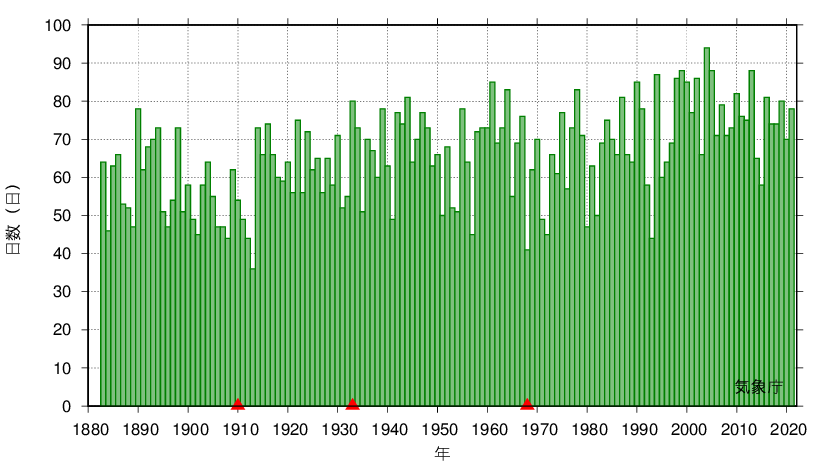
\includegraphics[width=\linewidth]{img/OSAKA_tmaxGE30.png}
      \subcaption{大阪 真夏日}
      \label{subfig1:temp_osaka}
    \end{minipage}\\
    \begin{minipage}[b]{\linewidth}
      \centering
      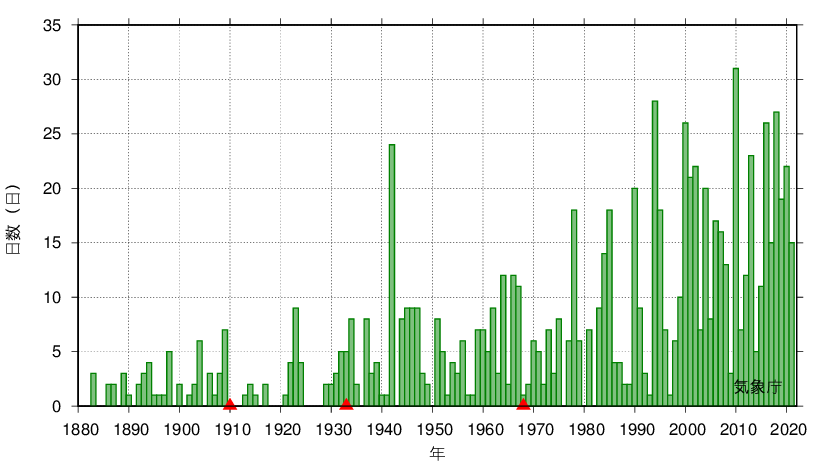
\includegraphics[width=\linewidth]{img/OSAKA_tmaxGE35.png}
      \subcaption{大阪 猛暑日}
      \label{subfig1:temp_osaka2}
    \end{minipage}
    \caption{真夏日および猛暑日の年間日数 1883-2021年\cite{temp_osaka3}}
    \label{fig1:temp_osaka}
\end{figure}
 

空調および冷凍分野において空気を冷やす原理として, "冷凍サイクル" が挙げられる. 
\figref{fig1:cycle}に示す通り, 冷凍サイクルは 「圧縮」「凝縮」「膨張」「蒸発」 
の4行程で構成されている. 冷凍サイクルにおいてモリエル線図(\figref{fig1:ph_r410}) 
は使用する冷媒の状態変化に伴う運転状況の変化, 装置能力, 装置動力などの計算に
よく使用される. 
前述した気温上昇に伴い, 今後は空調機の利用機会が増えると予想できる. 
一般に空調機には室内機と室外機に分類されており, 
冷房時において, 室外機は圧縮と凝縮, 室内機は蒸発と膨張の行程をそれぞれ担っている. 
室外機は高圧化した冷媒ガスを外気と熱交換させることで凝縮させ, 
室内機では, 膨張した冷媒液を室内の空気と熱交換させて冷媒の潜熱を利用して冷却する. 

\begin{figure}[htb]
  \centering
      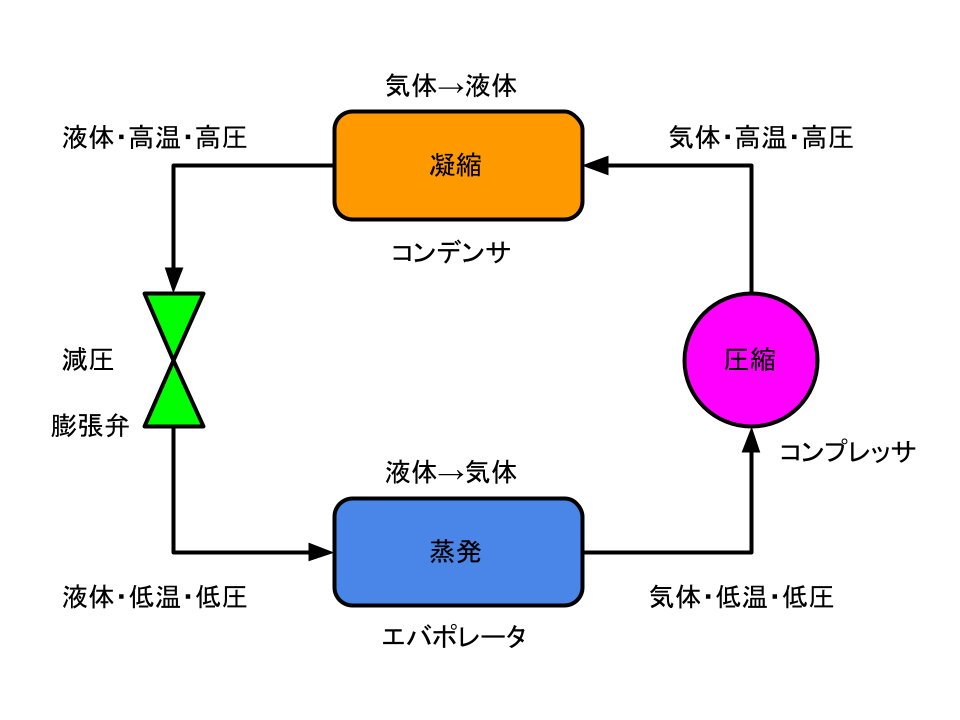
\includegraphics[width=0.8\linewidth]{img/cycle-2.png}
      \caption{冷凍サイクル}
      \label{fig1:cycle}
\end{figure}

\begin{figure}[htb]
    \centering
        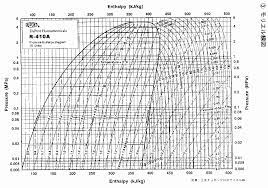
\includegraphics[width=\linewidth]{img/ph線図.jpg}
        \caption{モリエル線図(p-h 線図) 冷媒:R410}
        \label{fig1:ph_r410}
\end{figure}

ここで, 室外機吸い込み側空気, つまり外気温度が上昇すると, それに付随して凝縮温度
が高くなる. それにより冷却能力は小さくなり, 圧縮機駆動の駆動力が大きくなるため, 
成績係数が小さくなる. したがって, 同じ冷凍能力を出すためには消費電力が大きくなる.  
さらに, 空冷機の冷却温度は外気温度マイナス10$^\circ$Cが目安とされており, 猛暑日になると
室内が十分に冷えなくなるや高圧化防止のため運転が停止されるなどの問題もある. 
こういった問題を防止するために, 自動散水機などが市販でも販売されている(\figref{fig:truble_cut}). 

\begin{figure}[htb]
  \centering
  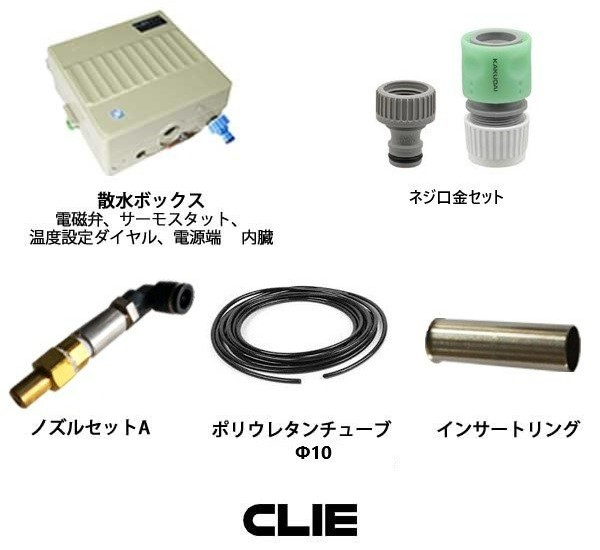
\includegraphics[width=0.8\linewidth]{img/trubleCut.jpg}
  \caption{㈱CLIE 室外機散水装置 トラブルカット\cite{clie}}
  \label{fig:truble_cut}
\end{figure}

実際に外気温30℃, 相対湿度50\%の環境下で簡易的な散水をしながら電力量を計測した. 
その対照実験の計測環境は\tableref{table:ex1}のとおりである. 
\figref{fig1:compare_watering}に示すように, 実験2 (散水あり) の電力量は実験1 (散水なし) のそれと
比較して小さくなっていることが分かる.

\begin{table}[htb]
  \caption{計測環境}
  \label{table:ex1}
  \centering
  \begin{tabular}{lcccc}
     & 外気温 & 湿度 & 設定温度 & 気候 \\[-1.5mm]
     & [$^\circ$C] & [\%] & [$^\circ$C] &  \\
    \hline \hline
    実験1 & 34.3 & 48.0 & 27.0 & 晴れ  \\
    実験2 & 32.9 & 58.9 & 27.0 & 曇り \\
    \hline
  \end{tabular}
\end{table}

\begin{figure*}[htb]
  \centering
      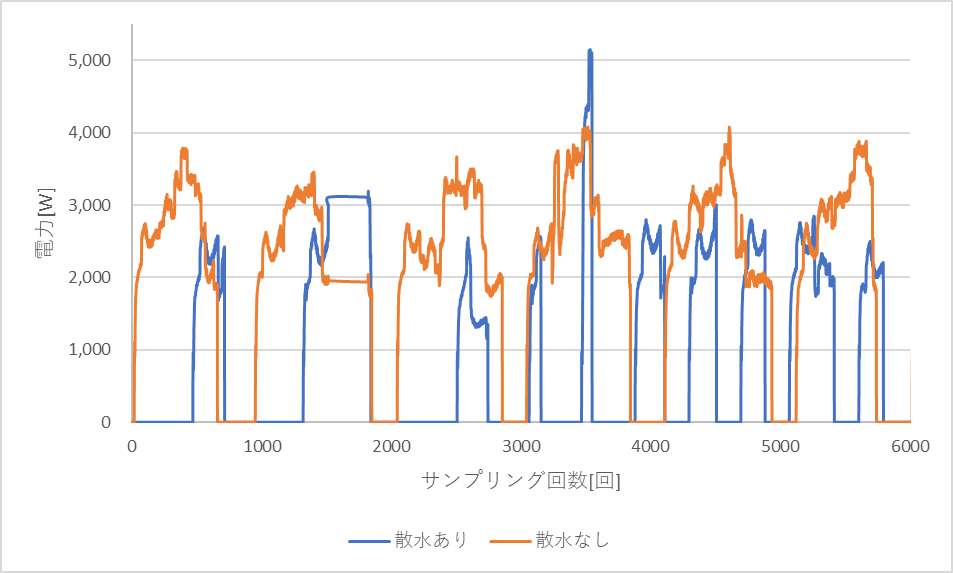
\includegraphics[width=0.8\linewidth]{img/ex1.png}
      \caption{散水の有無による電力量の比較}
      \label{fig1:compare_watering}
\end{figure*}


\subsection{目的}\label{purpose}
\subsecref{background} より, 室外機において散水システムの導入が効果的であるという事が分かった. 
そこで本研究では, 散水システムの導入に伴い自作散水システムや市販の機器など様々な条件で比較検証を行い, 
電気代および水道代とのコストバランスを考慮しながら, 最適な散水システムを検討することを目的とする. 

\section{調査内容}\label{sec2}
本章では本研究で行った計測のための調査内容について説明する. 

本研究で調査対象とした室外機はビル用マルチエアコンである三菱社 
PUHY-EP335DMG9\cite{condensing_unit}を採用した (\figref{fig:condensing_unit}, \tableref{table:hard}). 
この室外機に散水の有無など, 以下の4条件に分けて計測を行っていく.  

\begin{description}
  \item[  実験1.1 ] 散水なし
  \item[  実験1.2 ] 散水あり (手動)
  \item[  実験1.3 ] 散水あり (自作)
  \item[  実験1.4 ] 散水なし (雨天)
\end{description}

\begin{figure}[htb]
  \centering
  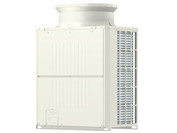
\includegraphics[width=0.7\linewidth]{img/PUHY-EP335DMG9.jpg}
  \caption{室外機 PUHY-EP355DMG9}
  \label{fig:condensing_unit}
\end{figure}

\begin{table}[htb]
  \caption{室外機仕様(冷房時)}
  \label{table:hard}
  \centering
  \begin{tabular}{lr}
    PUHY-EP355DMG9 & \\
    \hline \hline
    電源 & 3相 200V \\
    能力 & 33.5 kW \\
    消費電力 & 10.7 kW \\
    冷媒 & R410 \\
    \hline
  \end{tabular}
\end{table}



また、計測時間は日中で最も気温が高くなる13時から15時までの2時間とし, 
データログを取れるもの以外のパラメータは10分ごとに計測するとした. 


\subsection{自作散水システム}
本節では, 計測実験の比較対象として自作する散水システムの概要について説明する. 
屋上にある蛇口からホースと塩化ビニル管を結合させて室外機まで通し, 散水ノズルを
凝縮器側に左右3個ずつ計6個を設置した(\figref{fig2:watering_sys}). 

\begin{figure}[htb]
  \centering
    \begin{minipage}[b]{0.45\linewidth}
      \centering
      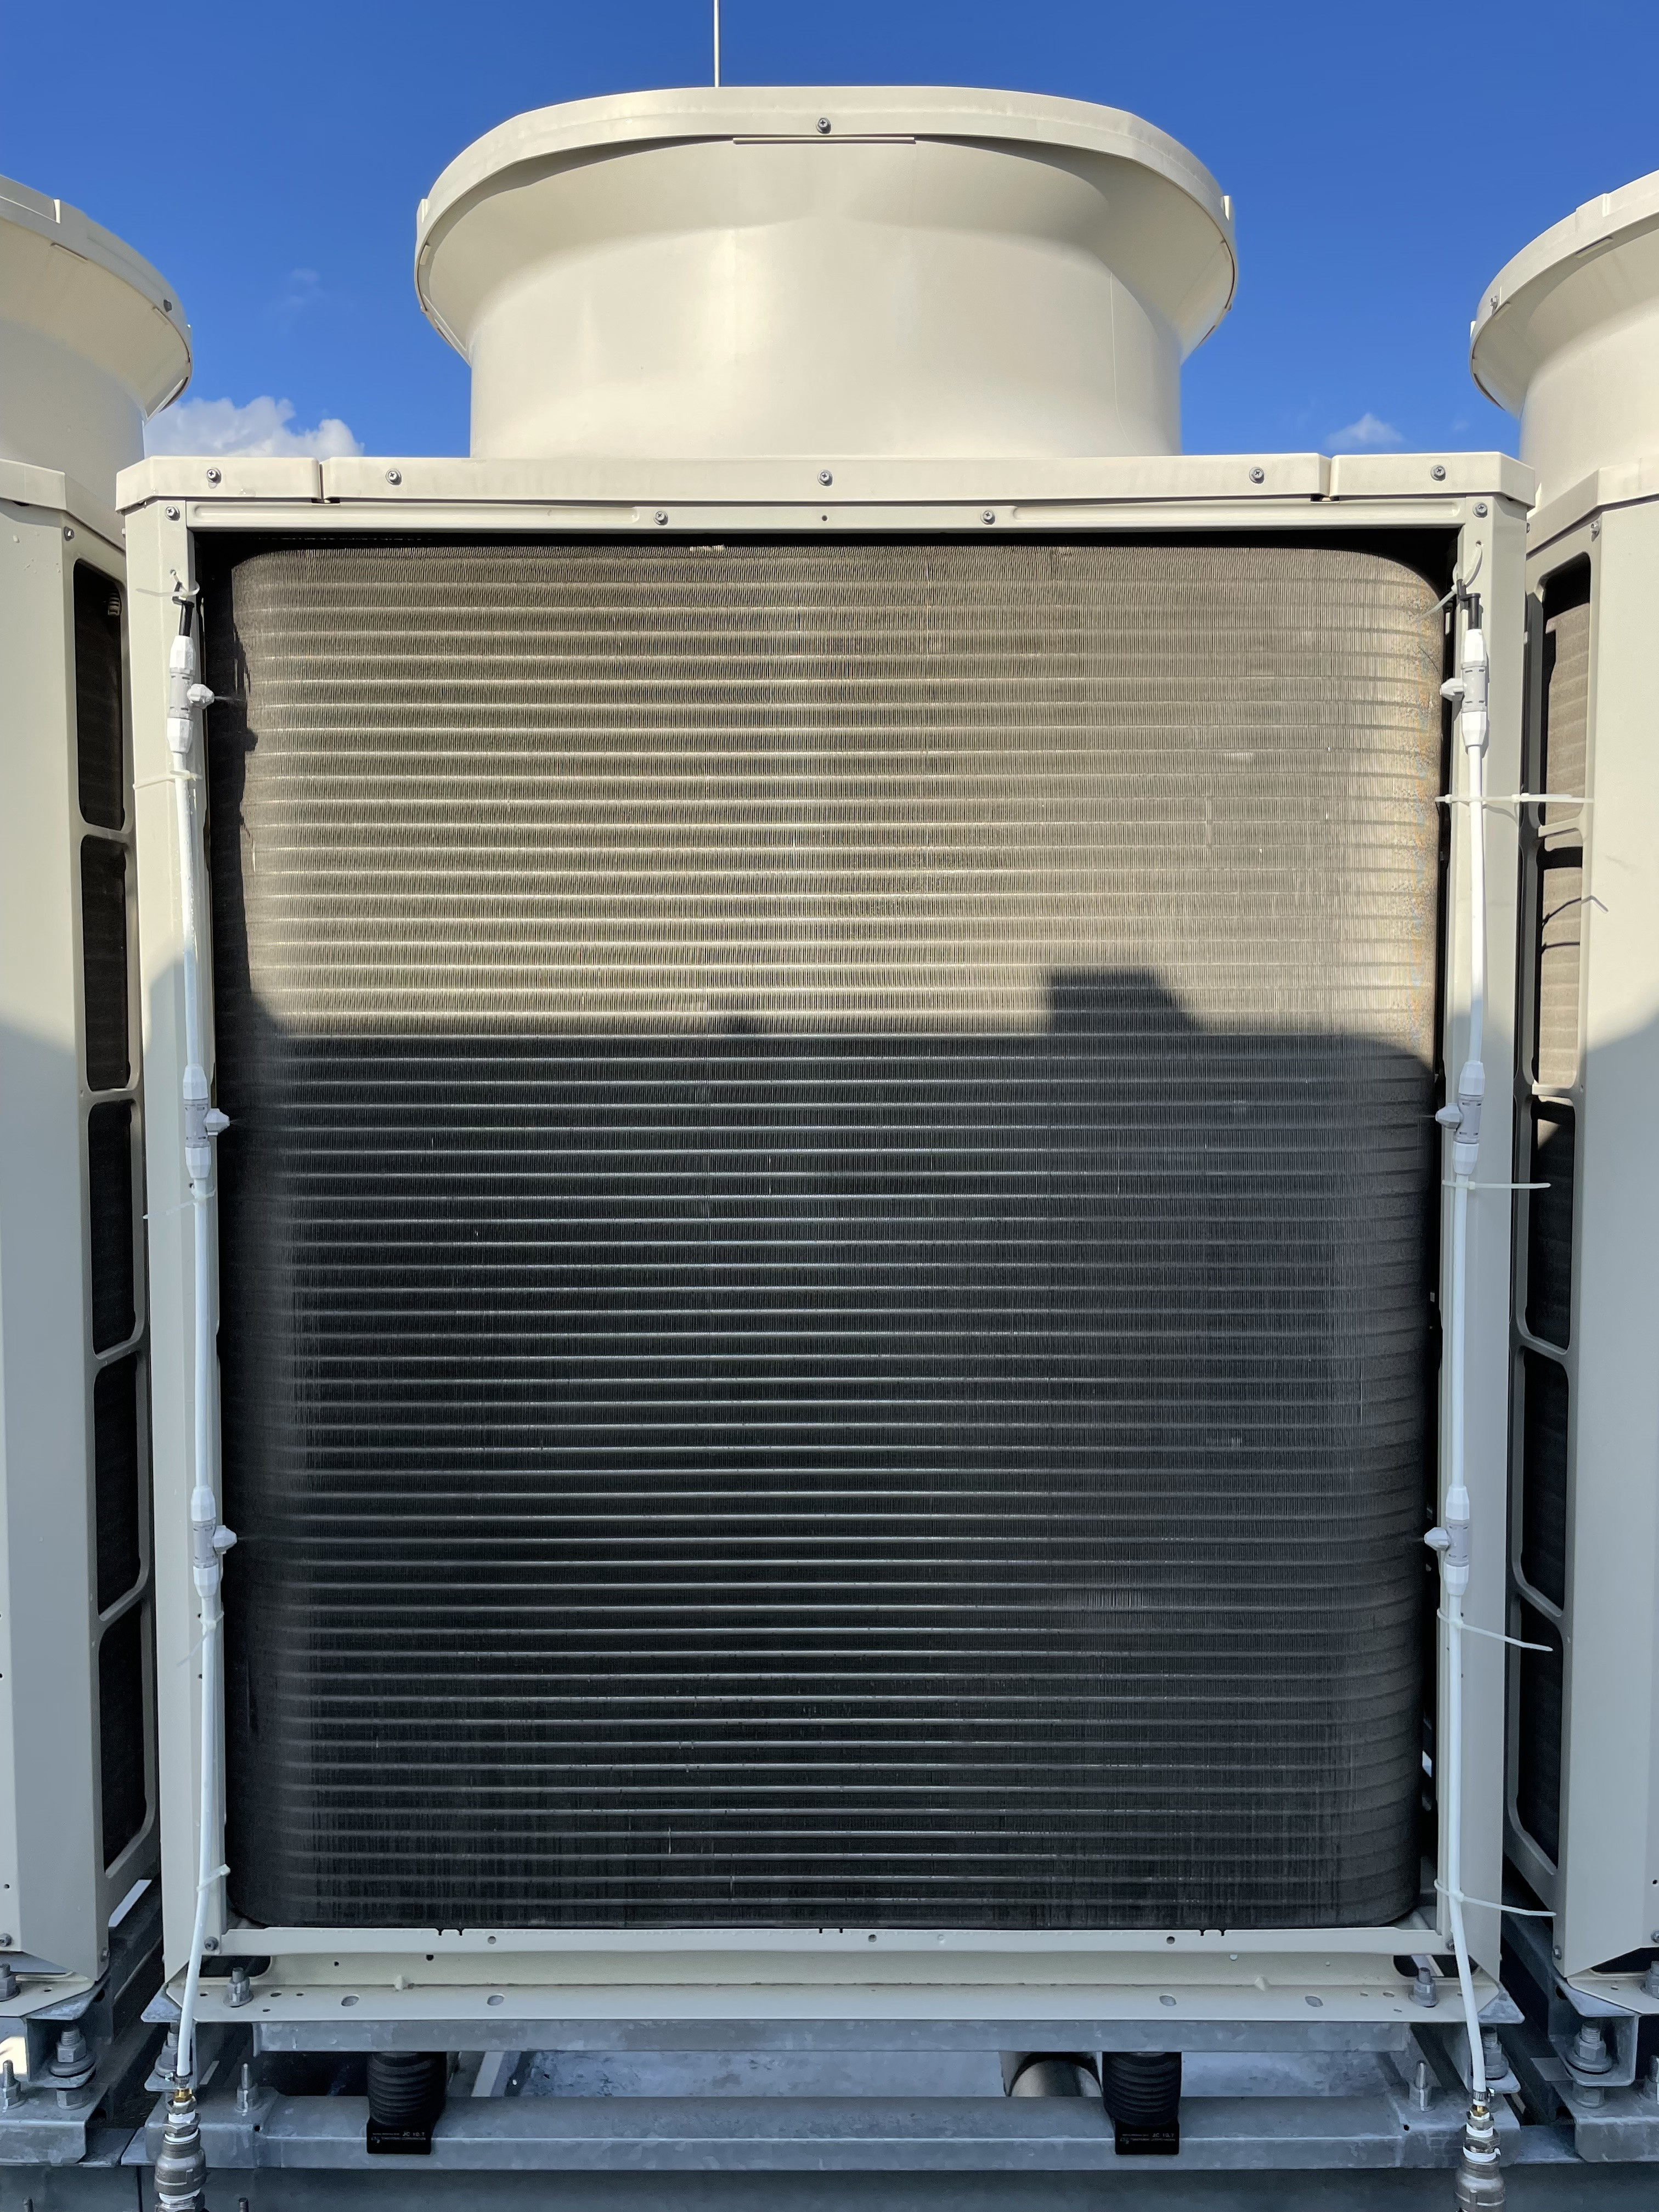
\includegraphics[width=\linewidth]{img/IMG_0146.jpg}
      \subcaption{凝縮器側}
    \end{minipage}
    \begin{minipage}[b]{0.45\linewidth}
      \centering
      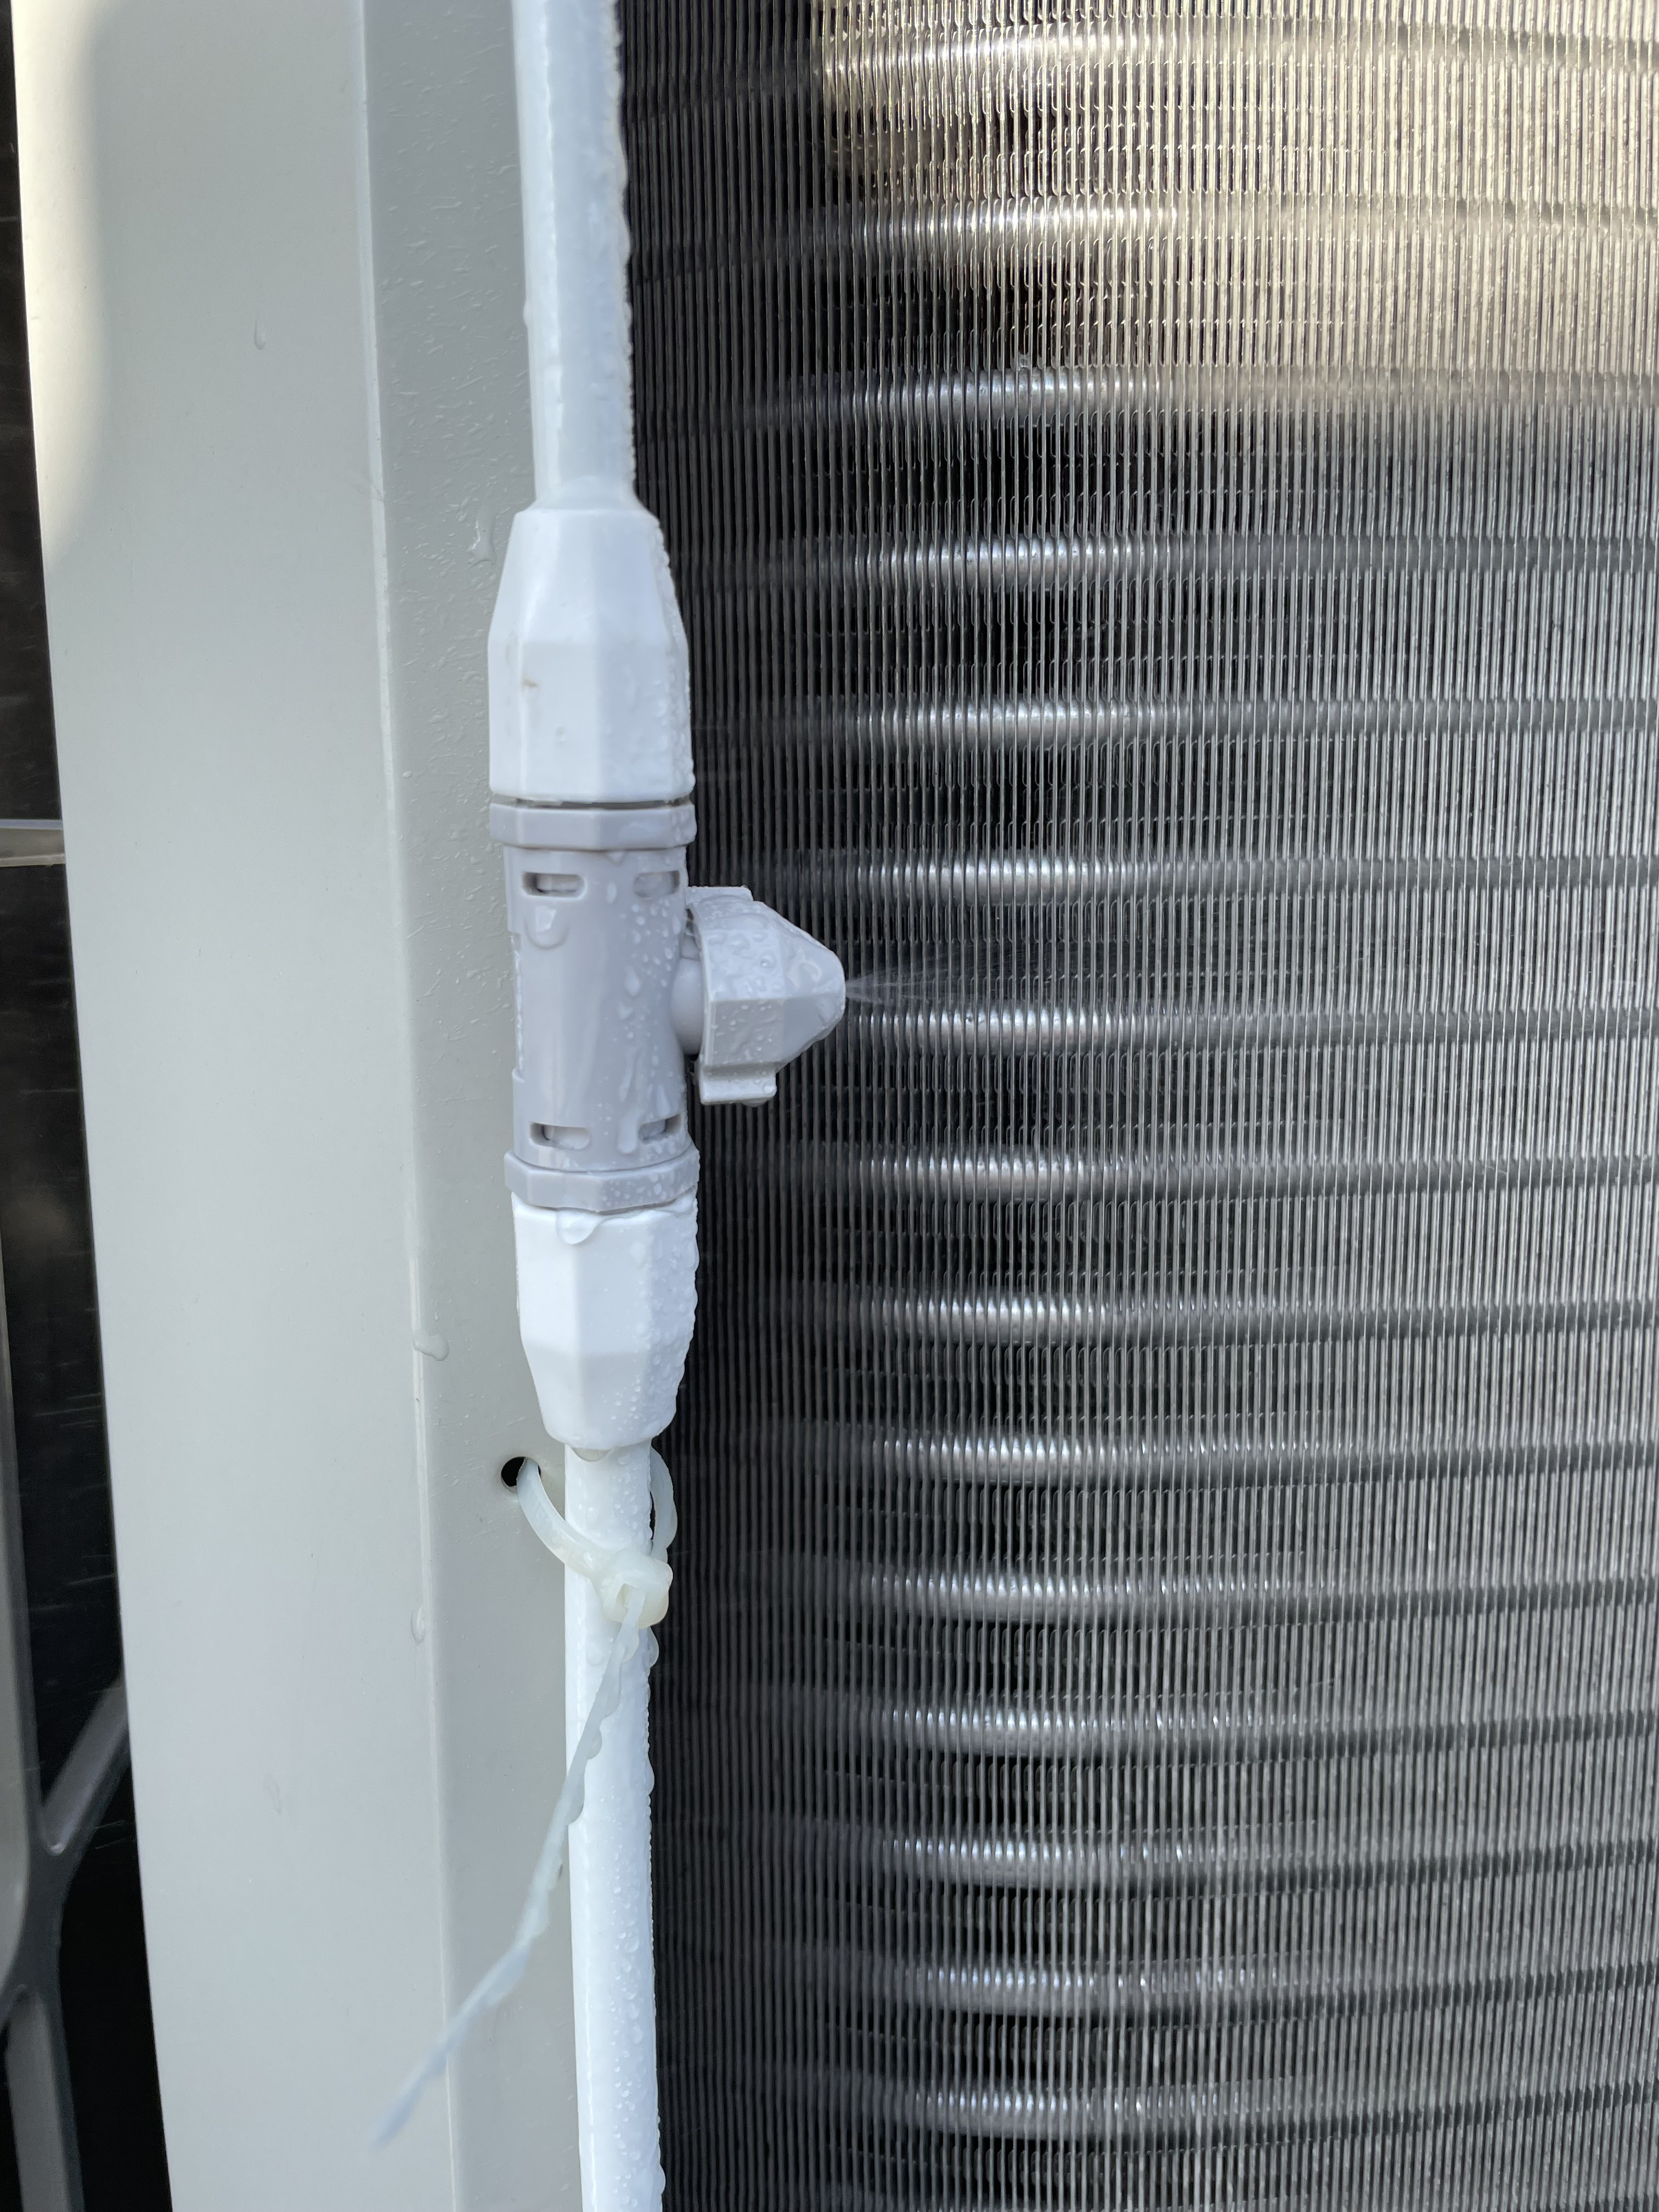
\includegraphics[width=\linewidth]{img/IMG_0142.jpg}
      \subcaption{散水用ノズル}
    \end{minipage}
  \caption{散水システム}
  \label{fig2:watering_sys}
\end{figure}

\subsection{計測}
実験で計測するパラメータは以下の通りである. 

\begin{itemize}
  \item 外気環境(気温, 相対湿度, 風速)
  \item 凝縮器入口温度 (2箇所)
  \item 凝縮器出口温度 (2箇所)
  \item 室外機 (圧縮機運転状況)
  \item 電気系 (電流, 電圧, 電力量)
  \item 散水系 (水温, 散水流量)
  \item 室内系 (設定温度, 温湿度)
\end{itemize}

これらのパラメータを各実験で比較, 得られた電力量の差について考察していく. 

\section{結果}\label{sec3}
各条件での計測結果は\tableref{table:ex}に示す通りである. 

\begin{table}[htb]
  \caption{実験の計測環境及び結果}
  \label{table:ex}
  \centering
  \begin{tabular}{crrrrr}
    \small 実験 & \small 計測日 & \small 気温 & \small 湿度 & \small 気候 & \small 設定温度 \\[-1.5mm]
     & & \small [$^\circ$C] & \small [\%] & & \small [$^\circ$C] \\
    \hline \hline
    1 & 7/13 & 34.3 & 48.0 & 晴れ & 26 - 27 \\
    2 & 7/15 & 32.9 & 58.9 & 曇り & 27.0 \\
    4 & 7/19 & 27.9 & 82.8 & 雨 & 27.0 \\
    3 & 7/23 & 33.2 & 43.4 & 晴れ & 27.0 \\
    5 & 7/21 & 32.1 & 58.4 & 曇り/雨 & 27.0 \\[2.5mm]
    6 & 7/25 & 36.5 & 42.2 & 晴れ & 25.0 \\
    7 & 7/26 & 37.5 & 41.0 & 晴れ & 25.0 \\
    \hline
  \end{tabular}
\end{table}

\begin{table}[htb]
  \caption{2時間あたりの電力量およびその他比較指標}
  \label{table:ex2}
  \centering
  \begin{tabular}{crrrrr}
    \small 実験 &   \small 外気h & \small 消費電力 & \small 電気代 & \small 変化率\\[-1.5mm]
    & \small [kJ/kg] & \small [kWh] & \small [円] & \small [\%] \\
    \hline \hline
    27℃ \\
    \hline
    1 & 76.5 & 4.24 & 118 & ― \\
    2 & 80.9 & 1.66 & 42 & 35.6 \\
    4 & 78.4 & 2.88 & 72 & 61.0 \\
    3 & 66.2 & 0.72 & 18 & 15.3 \\
    5 & 77.5 & 1.04 & 26 & 22.0 \\[2mm]
    25℃ \\
    \hline
    6 & 78.5 & 3.12 & 80 & ― \\
    7 & 80.6 & 4.45 & 112  & 140 \\
    \hline
  \end{tabular}
\end{table}

\begin{figure}[htb]
  \centering
  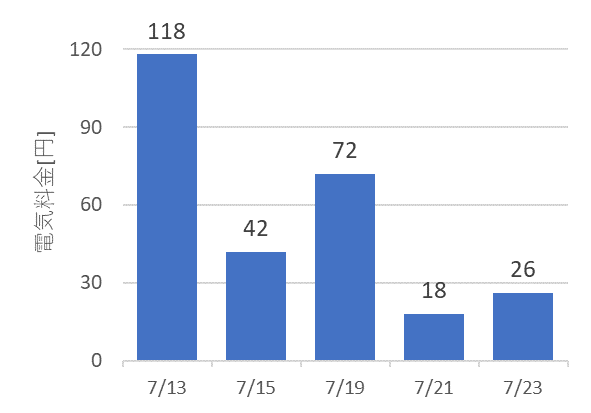
\includegraphics[width=\linewidth]{img/fee_27.png}
  \caption{電気料金比較 (実験グループ1)}
  \label{fig:fee_27}
\end{figure}

各計測実験での電力量との推移は\figref{fig1:compare_watering}に示す. 

従量電気料金を25円として見積もった際の各実験における2時間でかかった電力量
および電気代は\tableref{table:ex2}および\figref{fig:fee_27}に示す. 


% 仮挿入
\begin{figure*}[htb]
  \centering
    \begin{minipage}[b]{0.45\linewidth}
      \centering
      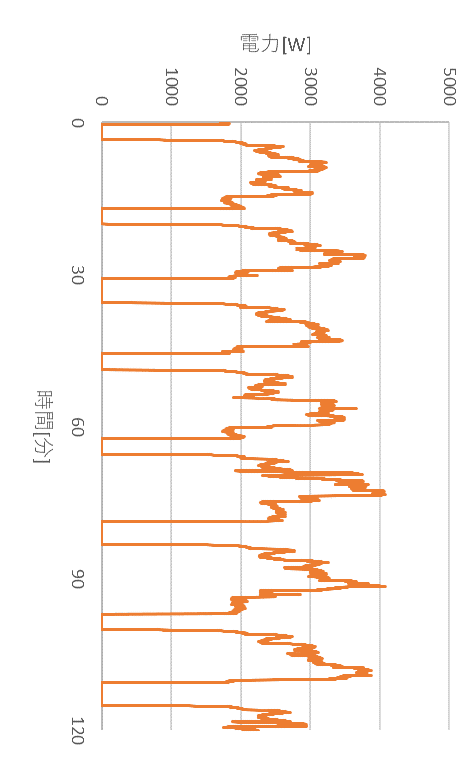
\includegraphics[width=\linewidth]{img/0713_power.png}
      \subcaption{実験1(27℃ 散水なし)}
    \end{minipage}
    \begin{minipage}[b]{0.45\linewidth}
      \centering
      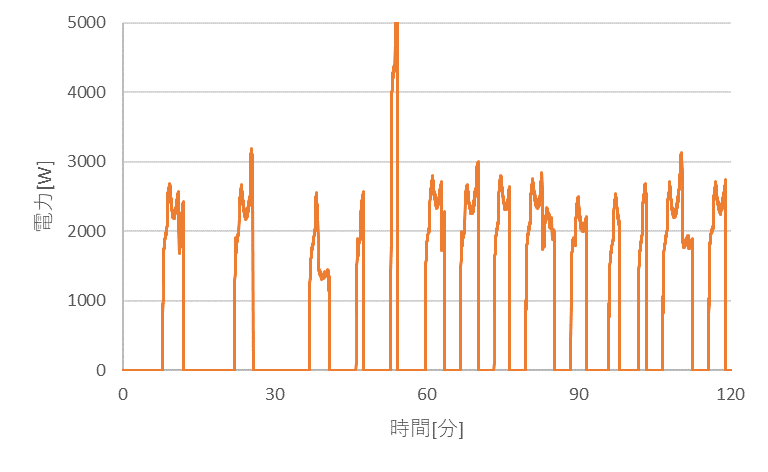
\includegraphics[width=\linewidth]{img/0715_power.png}
      \subcaption{実験2(27℃ 手動散水)}
    \end{minipage}\\
    \begin{minipage}[b]{0.45\linewidth}
      \centering
      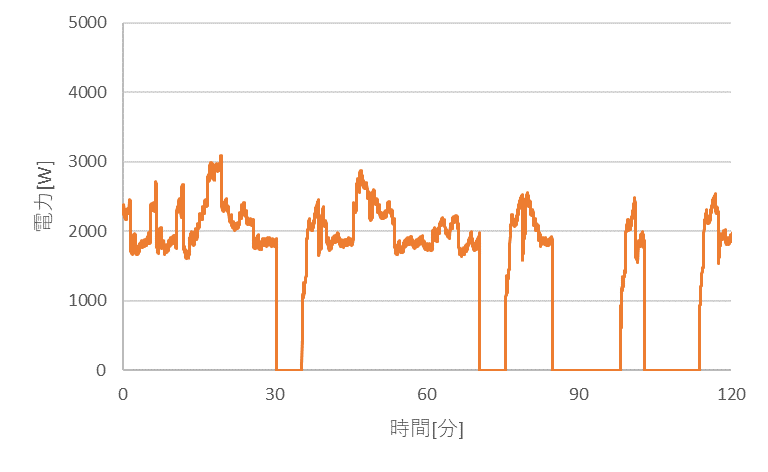
\includegraphics[width=\linewidth]{img/0719_power.png}
      \subcaption{実験3(27℃ 雨天)}
    \end{minipage}
    \begin{minipage}[b]{0.45\linewidth}
      \centering
      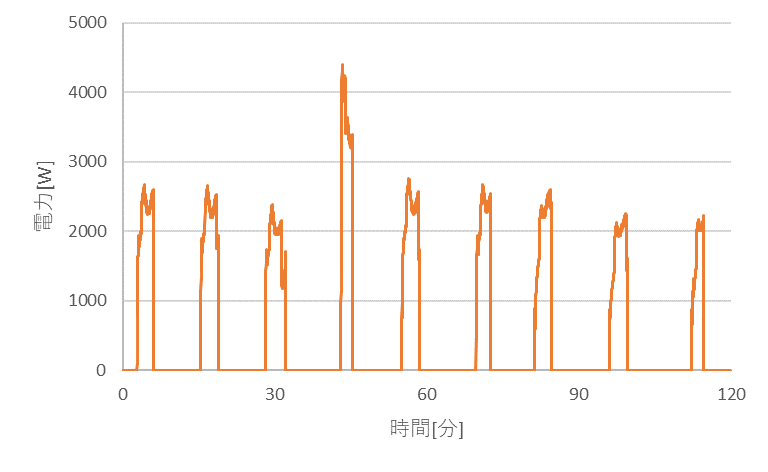
\includegraphics[width=\linewidth]{img/0721_power.png}
      \subcaption{実験4(27℃ 手動散水)}
    \end{minipage}\\
    \begin{minipage}[b]{0.45\linewidth}
      \centering
      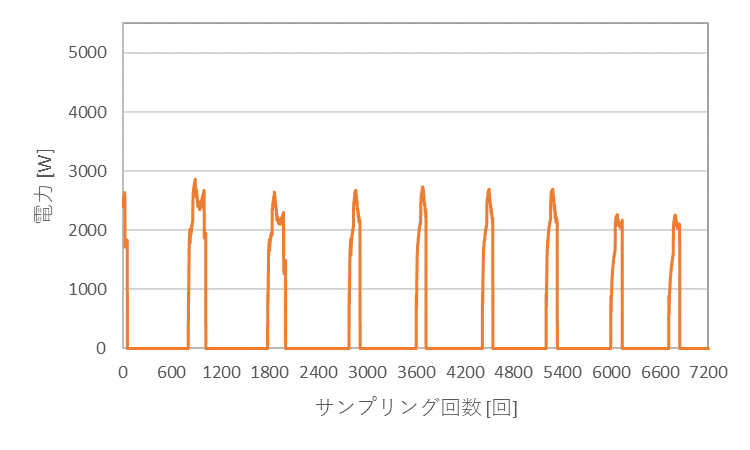
\includegraphics[width=\linewidth]{img/0723_power.png}
      \subcaption{実験5(27℃ 手動散水)}
    \end{minipage}
    \begin{minipage}[b]{0.45\linewidth}
      \centering
      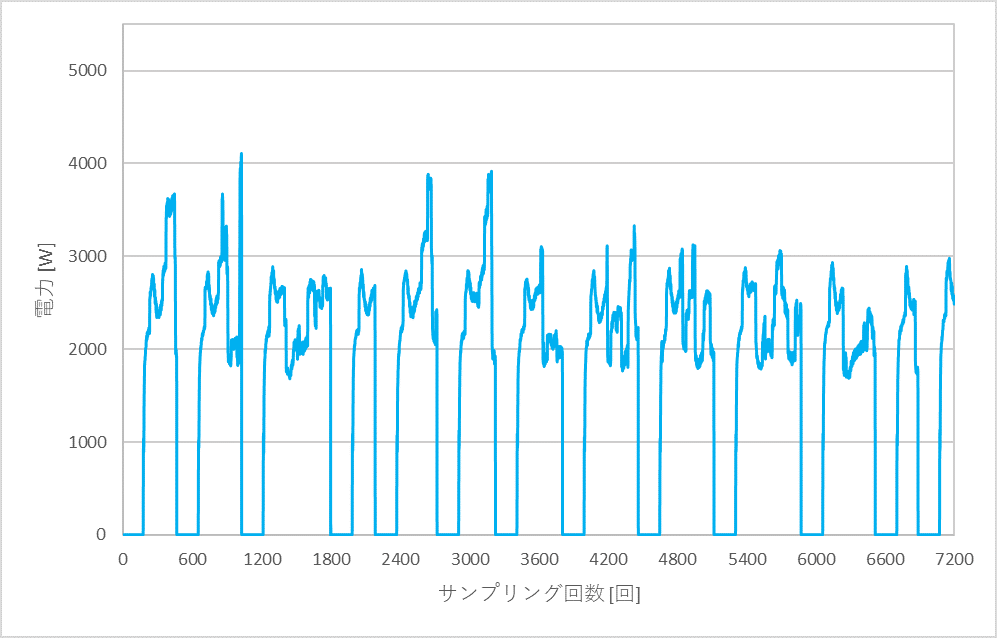
\includegraphics[width=\linewidth]{img/0725_power.png}
      \subcaption{実験6(25℃ 散水なし)}
    \end{minipage}\\
    \begin{minipage}[b]{0.45\linewidth}
      \centering
      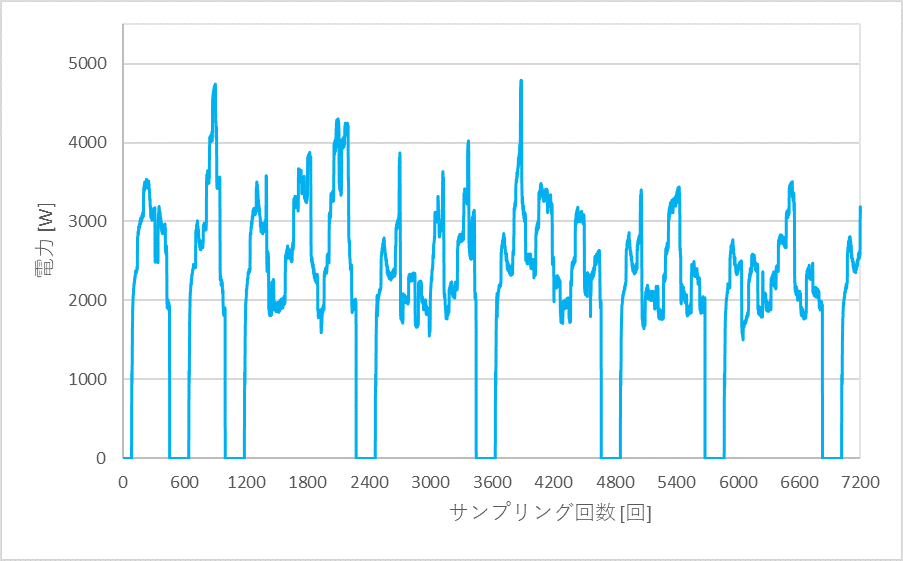
\includegraphics[width=\linewidth]{img/0726_power.png}
      \subcaption{実験7(25℃ 自動散水)}
    \end{minipage}
  \caption{電力量推移}
  \label{fig2:ex_outputs}
\end{figure*}

\section{考察}
(挿入したグラフ)に示す通り, 散水した場合は最大消費電力および運転時間が
小さくなっている事が分かる. 
\tableref{table:electric_bill}から, 実験1に比べた消費電力の減少率は, 実験2で約60\%, 
実験4で約32\% 減少することが分かった. 
これらの値は外気環境が異なるため, 正当性の評価としては難しい面があるが, 大まかな比較として
電力量が減少していることが分かる. 

また, 散水ありの場合でも, 手動で行った場合と自動機器を用いて散水した場合では
〇〇\% 減少率に偏差が生まれた. これは散水量と散水範囲の違いも考慮できるが, 
大部分は, 紙コップで散水したのに対し, ノズルによる散水は粒子の大きさが小さいために
水の潜熱による凝縮器吸込温度の低下が効率良く行えたことによるものが大きいと考えられる. 
今回手動の散水では約〇〇Lの水を1分間かけて散水するのを2回行ったが, 十分効果があるため, 
機器の導入が難しい場合であっても有効な手段であると考える. 
しかし, 散水は炎天下のなか行う場合が多いため, 担当者の負担と人的コストと考慮すると賢明な
判断とは言い難い. 

本州などの比較的平均気温の高い地域では, 導入におけるイニシャルコストは
約〇〇ヶ月で償却できるであろう. 

\section{結論}
本章では計測結果および考察を総括した結論を示す. 

%参考文献
\begin{thebibliography}{99}
\bibitem{temp_osaka}
国土交通省, 気象庁, 大阪府 日最高気温の月平均値, 
\url{https://www.data.jma.go.jp/obd/stats/etrn/view/monthly_s3.php?prec_no=62&block_no=47772&year=&month=&day=&view=a2}\vspace{2mm}

\bibitem{temp_osaka2}
George's Web Sites, 大阪府-大阪市の気温に関する統計情報, 
\url{http://www.tvg.ne.jp/george/weather/gw_stat_temp.html?city=oosaka}\vspace{2mm}

\bibitem{temp_osaka3}
A-PLAT 気候変動適応プラットフォーム, 気候変動の観測・予測データ, 大阪府観測データ, 
\url{https://adaptation-platform.nies.go.jp/map/Osaka/index_past.html}\vspace{2mm}

\bibitem{condensing_unit}
三菱電機, 暮らしと設備の業務サイト WIN2K, ビル用マルチエアコン 室外ユニット PUHY-EP335DMG9, 
\url{https://www.mitsubishielectric.co.jp/ldg/wink/ssl/displayProduct.do?pid=317186&ccd=2020121158}\vspace{2mm}

\bibitem{clie}
株式会社クリエ, 高圧カット防止室外機散水装置 トラブルカット, 
\url{https://c-clie.shop-pro.jp/?pid=134166927}\vspace{2mm}

\end{thebibliography}
%
%
%
\end{document}